\documentclass[11pt,a4paper]{article}
\usepackage[utf8]{inputenc}
\usepackage[margin=1in]{geometry}
\usepackage{graphicx}
\usepackage{hyperref}
\usepackage{xcolor}

\begin{document}
\noindent\textbf{\Large Tech Nation Visa - Exceptional Promise}\\
\noindent\textbf{Criteria:} Optional Criteria 3 (Significant Technical and Entrepreneurial Contribution)\\
\noindent\textbf{Applicant:} Odeyemi Olusegun Israel\\
\rule{\textwidth}{0.4pt}

\vspace{0.5cm}
\begin{center}
    \textbf{\huge Evidence 10: Cross-Chain Interoperability \& SDK Distribution}
\end{center}
\vspace{0.5cm}

\section*{1. Executive Summary}
\textbf{I built:} compliance enforcement across seven simultaneous blockchain networks --- closing the cross-chain evasion gap where a blacklisted wallet moves freely to a different chain --- and two developer SDKs that compress third-party integration from weeks of custom infrastructure work to hours, exposing nine specialist AI compliance services behind a single import.

\textbf{The problem:} conventional compliance tools enforce rules on one blockchain. A blacklisted wallet simply moves assets to a different network and transacts freely. I solved this by propagating risk scores and block decisions across seven networks via LayerZero (a cross-blockchain messaging protocol that transmits signed data packets between networks) --- a wallet blocked anywhere is blocked everywhere. EVM (Ethereum Virtual Machine) is the shared code standard across Ethereum, Polygon, Arbitrum, Optimism, Base, BSC, and Avalanche, meaning enforcement code written once applies to all of them.

Two developer SDKs --- TypeScript (\texttt{@amttp/client-sdk}) and Python (\texttt{amttp}) --- accompany the core system, exposing the full compliance stack behind a simple import. Neither wraps an existing library; both were written from scratch.

\vspace{0.3cm}
\noindent\textbf{Cross-Chain Contract Integration} (from \texttt{contracts/AMTTPCrossChain.sol}):

\vspace{0.2cm}
\noindent\fbox{\begin{minipage}{0.95\textwidth}
\small
\texttt{contract AMTTPCrossChain is Initializable, OwnableUpgradeable,}\\
\texttt{~~~~UUPSUpgradeable, ILayerZeroReceiver \{}\\[4pt]
\texttt{~~~~mapping(address => mapping(uint16 => uint256))}\\\texttt{~~~~~~~~public crossChainRiskScores;}\\
\texttt{~~~~mapping(address => bool) public globallyBlocked;}\\
\texttt{~~~~ILayerZeroEndpoint public lzEndpoint;}\\[4pt]
\texttt{~~~~function sendRiskScore(}\\
\texttt{~~~~~~~~uint16 \_dstChainId, address \_targetAddress,}\\
\texttt{~~~~~~~~uint256 \_riskScore, bytes calldata \_adapterParams}\\
\texttt{~~~~) external payable whenNotPaused nonReentrant \{}\\
\texttt{~~~~~~~~require(\_riskScore <= 1000, "Invalid risk score");}\\
\texttt{~~~~~~~~bytes memory payload = abi.encode(}\\
\texttt{~~~~~~~~~~~~MSG\_RISK\_SCORE, \_targetAddress, \_riskScore);}\\
\texttt{~~~~~~~~lzEndpoint.send\{value: msg.value\}(}\\
\texttt{~~~~~~~~~~~~\_dstChainId, trustedRemotes[\_dstChainId],}\\
\texttt{~~~~~~~~~~~~payload, payable(msg.sender), address(0),}\\
\texttt{~~~~~~~~~~~~\_adapterParams);}\\
\texttt{~~~~\}}\\
\texttt{\}}
\end{minipage}}
\vspace{0.2cm}

\noindent\textit{Figure 1: \texttt{AMTTPCrossChain.sol} --- upgradeable Solidity contract implementing LayerZero cross-chain message passing. A risk score or block decision on one of 7 EVM networks is encoded, signed, and broadcast to all connected chains. \texttt{nonReentrant} and \texttt{whenNotPaused} guards prevent replay and denial-of-service.}

\section*{2. Developer SDK Distribution}
Two developer integration kits were designed and released alongside the core system:
\begin{itemize}
    \item \textbf{TypeScript SDK} (\texttt{@amttp/client-sdk}): For web and application developers. Provides AI-powered risk scoring, blockchain enforcement integration, identity compliance checks, and support for multiple blockchain networks, accessible in a few lines of code.
    \item \textbf{Python SDK} (\texttt{amttp}): For data scientists and backend engineers. Provides the same capabilities using the Python programming language, which is standard in financial analytics and data science teams.
\end{itemize}

\vspace{0.3cm}
\noindent\textbf{TypeScript SDK Example} (from \texttt{packages/client-sdk/README.md}):

\vspace{0.2cm}
\noindent\fbox{\begin{minipage}{0.95\textwidth}
\small
\texttt{import \{ MLService, PolicyAction, utils \} from '@amttp/client-sdk';}\\[4pt]
\texttt{const mlService = new MLService('http://localhost:8000');}\\[4pt]
\texttt{const risk = await mlService.scoreTransaction('tx\_001', \{}\\
\texttt{~~amount: 1.5,~~~~~~~~~// ETH}\\
\texttt{~~velocity\_24h: 3,}\\
\texttt{~~account\_age\_days: 90,}\\
\texttt{\});}\\[4pt]
\texttt{console.log(`Risk: \$\{utils.formatRiskScore(risk.riskScore)\}`);~~// "97.2\%"}\\
\texttt{console.log(`Action: \$\{PolicyAction[risk.action]\}`);~~~~~~~~~~~~// "ESCROW"}
\end{minipage}}

\vspace{0.3cm}
\noindent\textbf{Python SDK Example} (from \texttt{packages/python-sdk/README.md}):

\vspace{0.2cm}
\noindent\fbox{\begin{minipage}{0.95\textwidth}
\small
\texttt{from amttp import AMTTPClient, AMTTPConfig}\\[4pt]
\texttt{config = AMTTPConfig(}\\
\texttt{~~rpc\_url="https://mainnet.infura.io/v3/YOUR\_KEY",}\\
\texttt{~~oracle\_url="https://oracle.amttp.io",}\\
\texttt{~~ml\_api\_url="https://ml.amttp.io",}\\
\texttt{)}\\[4pt]
\texttt{client = AMTTPClient(config)}\\
\texttt{risk = client.score\_transaction(}\\
\texttt{~~to="0x742d35Cc...", value=1\_000\_000\_000\_000\_000\_000,}\\
\texttt{~~features=\{"velocity\_24h": 5, "account\_age\_days": 30\}}\\
\texttt{)}\\[4pt]
\texttt{print(f"Risk Score: \{risk.risk\_score:.2\%\}")~~~~\# "Risk Score: 94.12\%"}\\
\texttt{print(f"Action: \{risk.action.name\}")~~~~~~~~~~~~\# "Action: ESCROW"}
\end{minipage}}
\vspace{0.2cm}

\noindent\textit{Figure 2: TypeScript and Python SDK quick-start examples. A third-party developer can score a transaction against AMTTP's full compliance stack --- ML risk, FCA sanctions, policy engine, and cross-chain data --- in under 10 lines of code in their preferred language. The Python SDK targets financial analytics teams; the TypeScript SDK targets web and application developers.}

\vspace{0.3cm}
\begin{center}
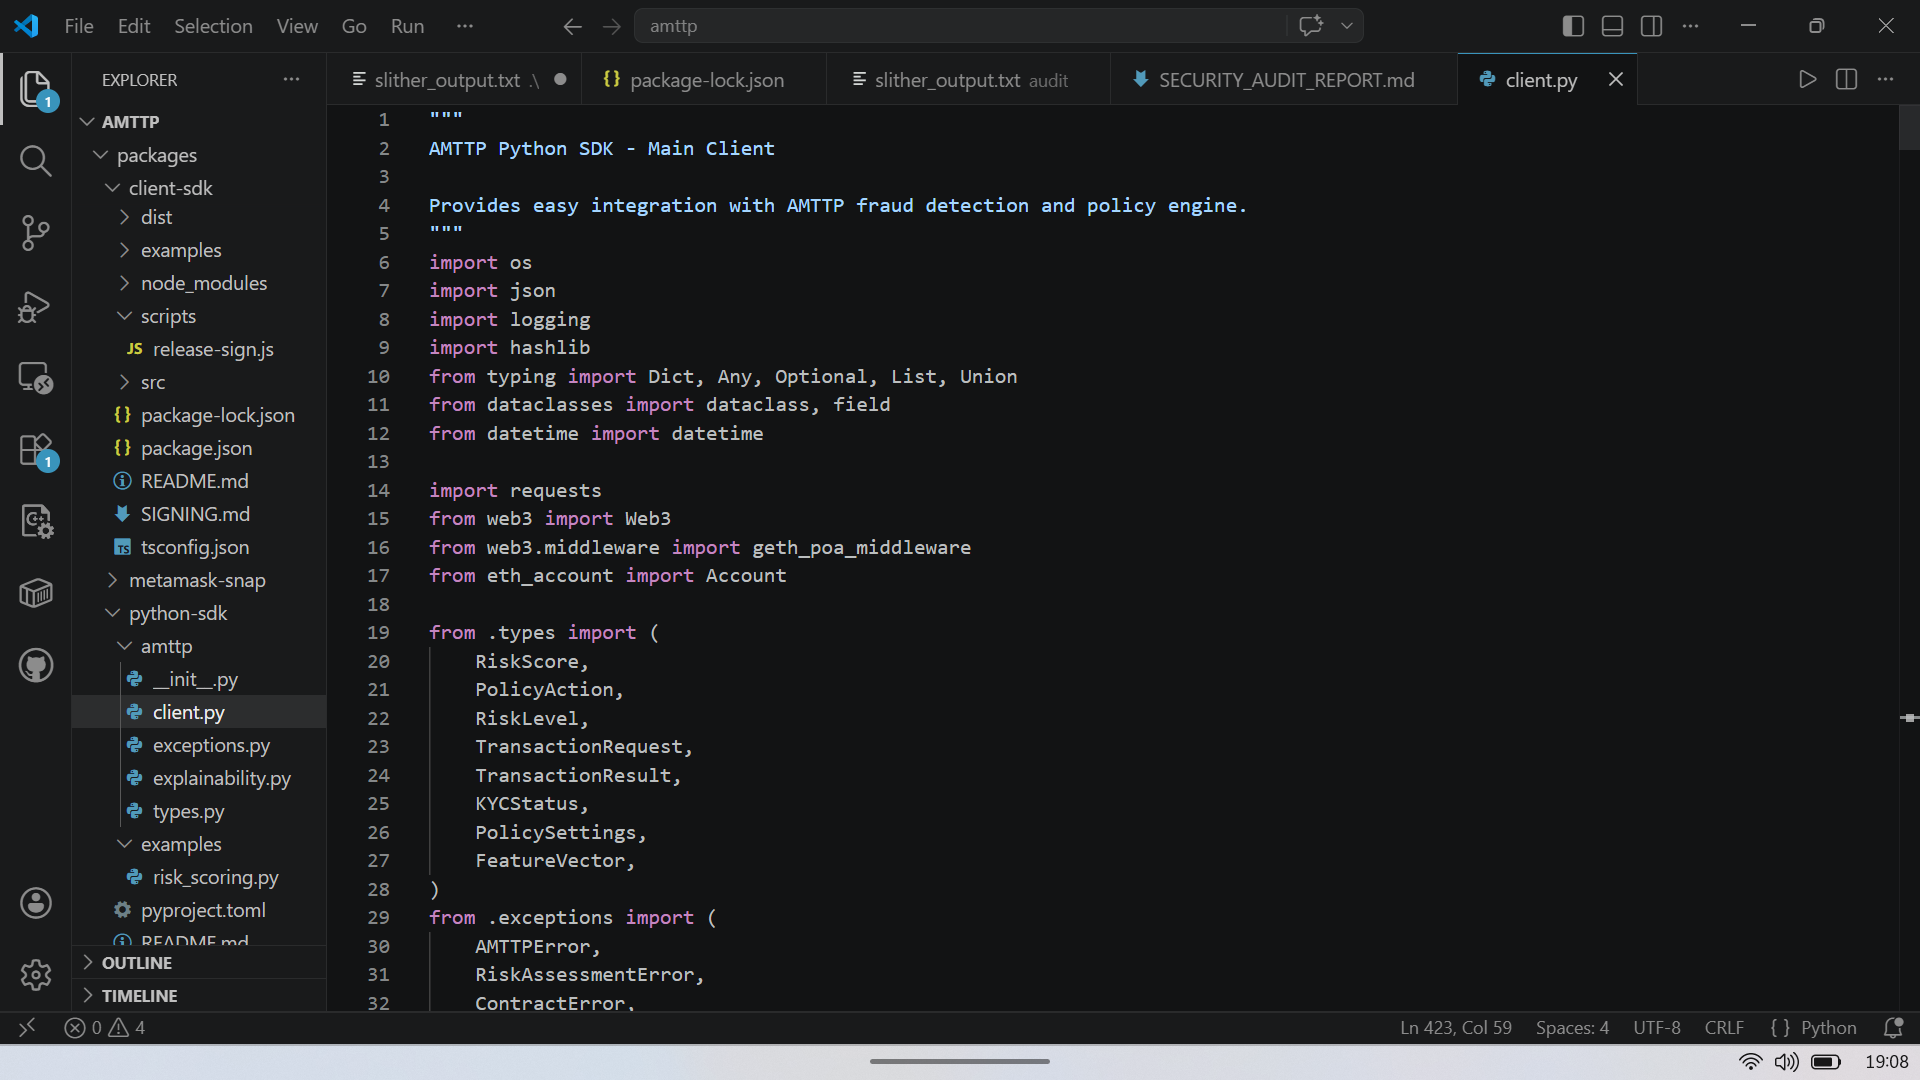
\includegraphics[width=0.95\textwidth]{images/vscode_sdk_packages.png}
\end{center}
\noindent\textit{Figure 3: VS Code workspace showing both SDKs fully structured and ready for distribution. Both packages are sole-authored: no collaborative commits, no fork from an existing open-source SDK. Each wraps the full nine-service AMTTP compliance stack behind a single import.}

\section*{3. Commercial Readiness and UK Ecosystem Value}
Cross-chain enforcement and distribution-ready SDKs transform AMTTP from a research system into a deployable compliance product. The architectural decision to implement enforcement at the cross-chain messaging layer --- rather than as a post-settlement reporting tool --- means a block decision propagates to all seven networks within the same transaction cycle. A wallet cannot evade by moving chains.

The two SDKs directly address the principal integration barrier for regulated institutions: a bank, payment processor, or fintech operating on any of the seven supported networks can integrate the full nine-service compliance stack within hours, in their preferred language, without rebuilding or understanding the underlying infrastructure. This eliminates a cost and complexity barrier that would otherwise require a dedicated blockchain engineering team. For UK digital-finance institutions operating under FCA digital-asset rules, Travel Rule obligations, or MiCA cross-border requirements, the enforcement layer and its distribution tooling represent production-ready infrastructure they can adopt immediately. I designed, built, and sole-authored every component.

\end{document}